\begin{frame}{SimDyNetKAT}
    \begin{itemize}
        \item A simplified version of DyNetKAT
        \item Replacing NetKAT terms with a sum of packet flows
    \end{itemize}
    \begin{align*}
        D & ::= \bot | F;D | x?F;D | x!F;D | D \parallel D
        | D \oplus D                                       \\
        F & ::= \alpha\cdot \pi
    \end{align*}
\end{frame}

\begin{frame}{Goals}
    \begin{itemize}
        \item Goal: Causal analysis of property violation in SimDyNetKAT
        \item Event structure semantic for SimDyNetKAT terms
        \item Event structure semantic for property violation
        \item Causal model for property violation in event structure
        \item Applying the analysis on some categories of network
              properties
        \item \textcolor{red} {Compositional causal analysis in
                  event structure}
    \end{itemize}
\end{frame}

\begin{frame}{Event Structure}
    An event structure is a triple $(E,\#,\vdash)$ where:
    \begin{itemize}
        \item $E$ is a set of events
        \item $\#$ is the binary symmetric, irreflexive conflict relation
        \item $\vdash \subseteq Con \times E$ is the enabling relation where:
              \begin{align*}
                  X   & \vdash e \wedge X \subseteq Y \in Con
                  \Rightarrow Y \vdash e                                      \\
                  Con & = \s{X \subseteq E| \forall e,e' \in X. \neg(e \#e')}
              \end{align*}
    \end{itemize}
\end{frame}

\begin{frame}{Labeled Event Structure}
    A labeled event structure is a tuple $(E,\#,\vdash,L,l)$
    where:
    \begin{itemize}
        \item $(E,\#,\vdash)$ is an event structure
        \item $L$ is a set of labels
        \item $l$ is a function $l : E \rightarrow L$
    \end{itemize}
\end{frame}

\begin{frame}{Labeled Event Structure Semantics for SimDyNetKAT}
    \begin{itemize}
        \item $\mathcal{A}$ is an alphabet of letters of the form
              $\alpha\cdot\pi$, $x?F$ and $x!F$
        \item $a \in \mathcal{A}$ and $\mathcal{L} \subseteq \mathcal{A}$
        \item $t$ is a SimDyNetKAT term
    \end{itemize}
    \begin{align*}
        \sem{\bot}              & = (\e)                                \\
        \sem{a;t}               & = a(\sem{t})                          \\
        \sem{t_1 \oplus t_2}    & = \sem{t_1} + \sem{t_2}               \\
        \sem{t_1 \parallel t_2} & = \sem{t_1} \times \sem{t_2}          \\
        \sem{\delta_{\mathcal{L}}(t)}
                                & = \sem{t}\lceil 
                                \Lambda_{ \mathcal{A} \setminus \mathcal{L}}
    \end{align*}

\end{frame}

\begin{frame}{Some Examples: Prefix}
    \begin{equation*}
        \begin{aligned}
            \mathcal{A} & = \s{a,b}           \\
            t           & = a;b               \\
            \sem{t}     & = (E,\#,\vdash,L,l) \\
        \end{aligned}
        \qquad \qquad
        \begin{aligned}
            E  & = \s{(0,a),(1,0,b)}                       \\
            \# & = \emptyset                               \\
               & \e \vdash (0,a), \s{(0,a)} \vdash (1,0,b) \\
            L  & = \s{a,b}                                 \\
               & l((0,a)) = a, l((1,0,b)) = b              \\
        \end{aligned}
    \end{equation*}
    \begin{align*}
    \end{align*}
    \begin{center}
        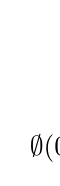
\begin{tikzpicture}[scale=0.8]
            \crd[right]{0}{0}{$\emptyset$}
            \crd[right]{0}{1}{$\s{(0,a)}$}
            \crd[right]{0}{2}{$\s{(0,a),(1,0,b)}$}
            \draw [ultra thick] (0,0) -- (0,1);
            \draw [ultra thick] (0,1) -- (0,2);
        \end{tikzpicture}
    \end{center}
\end{frame}

\begin{frame}{Some Examples: Sum}
    \begin{equation*}
        \begin{aligned}
            \mathcal{A} & = \s{a,b}           \\
            t           & = a+b               \\
            \sem{t}     & = (E,\#,\vdash,L,l) \\
        \end{aligned}
        \qquad \qquad
        \begin{aligned}
            E & = \s{(0,a),(1,b)}                \\
              & (0,a) \# (1,b) , (1,b) \# (0,a)  \\
              & \e \vdash (0,a), \e \vdash (1,b) \\
            L & = \s{a,b}                        \\
              & l((0,a)) = a, l((1,b)) = b       \\
        \end{aligned}
    \end{equation*}
    \begin{align*}
    \end{align*}
    \begin{center}
        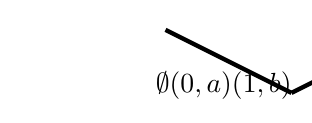
\begin{tikzpicture}[scale=0.8]
            \crd[above]{0}{0}{$\emptyset$}
            \crd[above]{-2}{1}{$\s{(0,a)}$}
            \crd[above]{2}{1}{$\s{(1,b)}$}
            \draw [ultra thick] (0,0) -- (-2,1);
            \draw [ultra thick] (0,0) -- (2,1);
        \end{tikzpicture}
    \end{center}
\end{frame}

\begin{frame}{Some Examples: Product}
    \begin{equation*}
        \begin{aligned}
            \mathcal{A} & = \s{a,b}           \\
            t           & = a \times b        \\
            \sem{t}     & = (E,\#,\vdash,L,l) \\
        \end{aligned}
        \qquad \qquad
        \begin{aligned}
            E  & = \s{(a,*),(*,b),(a,b)}                           \\
            \# & = \e                                              \\
               & \e \vdash (a,*), \e \vdash (*,b),\e \vdash (a,b)  \\
            L  & = \s{(a,*),(*,b),(a,b)}                           \\
               & l((a,*)) = (a,*), l((*,b)) = (*,b),l((a,b))=(a,b) \\
        \end{aligned}
    \end{equation*}
    \begin{align*}
    \end{align*}
    \begin{center}
        \begin{tikzpicture}[scale=0.8]
            \crd[above]{0}{0}{$\emptyset$}
            \crd[left]{-2}{1}{$\s{(a,*)}$}
            \crd[right]{2}{1}{$\s{(*,b)}$}
            \crd[above]{0}{2}{$\s{(a,*),(*,b)}$}
            \crd[above]{2}{3}{$\s{(a,b)}$}
            \draw [ultra thick] (0,0) -- (-2,1);
            \draw [ultra thick] (0,0) -- (2,1);
            \draw [ultra thick] (2,1) -- (0,2);
            \draw [ultra thick] (-2,1) -- (0,2);
            \draw [ultra thick] (0,0) -- (2,3);
        \end{tikzpicture}
    \end{center}
\end{frame}

\begin{frame}{Causal Model of Event Structure}
    \begin{itemize}
        \item Let $(E,\#,\vdash,L,l)$ be an event structure
              and         
              \item We define the causal model $M = (\mathcal{S},\mathcal{F},\mathcal{E})$
              to be the causal model of the violation in the given event structure

              \begin{align*}
                  \mathcal{S}     & = (\mathcal{U},\mathcal{V},\mathcal{R})  \\
                  \mathcal{V} =   & \s{C_{e_i,e_j} |  1 \leq i < j \leq n.
                  e_i \in E \amp e_j \in E}                                  \\
                                  & \cup \s{EN_{s,e} | s \in \mathcal{P}(E),
                  e \in E. e \not \in s }                                    \\
                                  & \cup \s{M_{s,e} | s \in \mathcal{P}(E),
                  e \in E. e \not \in s } \cup \s{PV}                     \\
              \end{align*}
    \end{itemize}
\end{frame}

\begin{frame}{Causal Model of Event Structure}
    $$
        \f{C_{e,e'}} = \begin{cases}
            true  & \text{ if } e \# e' \amp e' \# e \\
            false & \text{ otherwise }
        \end{cases}
    $$
    $$
        \f{M_{s,e}} = \begin{cases}
            Min(s,e) \wedge Con(s) & \text{ if } s \vdash_{min} e \\
            false                  & \text{ otherwise }
        \end{cases}
    $$
    \begin{align*}
        \f{EN_{s,e}} & = \left( M_{s,e} \vee
        \left( \bigvee_{s'\prec s}EN_{s',e} \right)
        \right) \bigwedge Con(s)
    \end{align*}
    \begin{align*}
        Con(s)   & =   \left(
        \bigwedge_{ 1\leq j<j' \leq n \wedge e_j,e_{j'} \in s}
        \neg C_{e_j,e_{j'}}
        \right)               \\
        Min(s,e) & = \left(
        \bigwedge_{s'. (s' \subset s \vee s \subset s')
            \wedge e \notin s'}
        \neg M(k',i)
        \right)
    \end{align*}
\end{frame}

\begin{frame}{Causal Model of Event Structure}
    Let $\mathbb{E}$ be the set of all event structures of the form
    $(E,\#',\vdash',L,l)$ where:
    \begin{itemize}
        \item $\#' \subseteq E \times E$
        \item $\vdash' \subseteq \mathcal{P}(E) \times E$
    \end{itemize}
    We define a function 
    $ES: \times_{V \in \mathcal{V}\setminus \s{PV}} \mathcal{R}(V) \rightarrow \mathbb{E}$
    which returns an event structure derived by values of variables
    Let $\vec v$ be the vector of values of variables in 
    $\mathcal{V} \setminus \s{PV}$
    we define $ES(\vec v) = (E,\#',\vdash', L,l)$ so that we have:
    \begin{align*}
        \forall e,e' \in E. e \#' e' \wedge e' \#' e
         & \iff \vec{v}(C_{e,e'}) = \T \\
        \forall s \in \mathcal{P}(E), e \in E.  s \vdash' e
         & \iff \vec{v}(EN_{s,e}) = \T
    \end{align*}
    We define $F_{PV}$ such that it encodes the safety property violation as a predicate on the set of configurations 
    of the given event structure
\end{frame}

\begin{frame}{Causal Model of Event Structure}
    Given an event structure $\mathrm{E} = (E,\#,\vdash,L,l)$
    and a safety violation encoded as $F_{PV}$, which is violated
    in $\mathrm{E}$, let $\mathcal{M}$ be the causal of the violation
    violation if the following three conditions hold:
    \begin{itemize}
        \item  \textbf{AC1.} $M\models \vec X = \vec x
                  \wedge PV = \T$.
        \item  \textbf{AC2. }There exists a partition $(\vec Z, \vec W)$ of $\mathcal{V}$ with $\vec X \subseteq \vec Z$ and some setting $(\vec x',\vec w')$ of the variables in $(\vec X,\vec W)$ such that if $(M,\vec u)\models \vec Z = z^*$ for all $Z\in \vec Z$, then both of the following conditions hold:

              (a) $M \models[\vec X \leftarrow \vec x', \vec W \leftarrow \vec w']
                  PV = \F
                  \wedge \vec V = \vec v
                  \wedge  \vec v \in \mathcal{E}$.

              (b) $M \models[\vec X\leftarrow \vec x, \vec W' \leftarrow \vec w', \vec Z'\leftarrow \vec z^*]
                  PV = \T
                  \wedge \vec V = \vec v
                  \wedge \vec v \in \mathcal{E}$
              for all subsets $\vec W'$ of $\vec W$ and all subsets $Z'$ of $\vec Z$.

        \item  \textbf{AC3.} $\vec X$ is minimal; no subset of $\vec X$ satisfies conditions $AC1$ and $AC2$.
    \end{itemize}
\end{frame}

\begin{frame}{Some Notation}
    Notation:
    \begin{itemize}
        \item In the following we assume a field $sw$ for the
        packet's switch
        \item We use $xy$ to denote $\alpha\cdot\pi$ where
            we have $sw = x$ in $\alpha$ and 
            $sw \la y$ in $\pi$

    \end{itemize}
\end{frame}